\section{PID Controller} %3.2
PID controller can be written in the following equation:

\begin{equation} \label{eq3}
u(t) = k_p e(t) + k_i \int_{0}^{t} e(\tau) d\tau + k_d \frac{d e}{d t}
\end{equation}

 where u is the control signal and e is the error. The nominal value is also called the reference value or the setpoint. The controller’s output is therefore summed by three terms: the P-term, the I-term, and the D-term. The P-term is proportional to the error and its amplification factor is $k_p$. The I-term is proportional to the integral of the error and its amplification factor is $k_i$. The D-term is proportional to the derivative of the error and its amplification factor is $k_d$. 
 
 The function of the P-term is trying to send a control signal proportional to the error. For example, there is a signal whose value is 90 and we hope it can approach to 100 using P-term only. The error now is (100 - 90 = 10). Assumed that $k_p$ equals to 0.5, then control signal becomes (10 x 0.5 = 5). The new signal becomes (90 + 5 = 95). If we continue to repeat this flow, we find the new signal turns to 97.5, 98.75 and 99.375. It seems like the new signal is approaching to our nominal value and it approach to the nominal value if we continue updating the signal. 
 

However, there are two situations that we cannot ignore. Firstly, steady-state error occurs if $k_p$ is not set well. For example, if $k_p$ equals to 2, the error be 20 and the new signal be 110, 90, 110, 90,… The signal can not be restored to the nominal one forever.  

The second situation is that, in reality, the signal is not perfect and it has its own errors. In the first example above, we choose 0.5 as our amplification factor ($k_p$) and thus the first new signal be 95. However, it is a possible the new signal will be lost its signal by 5 units every time after the control. Finally, the signal will remain 90 and the error will be 10.  

\begin{figure}[t]
\center
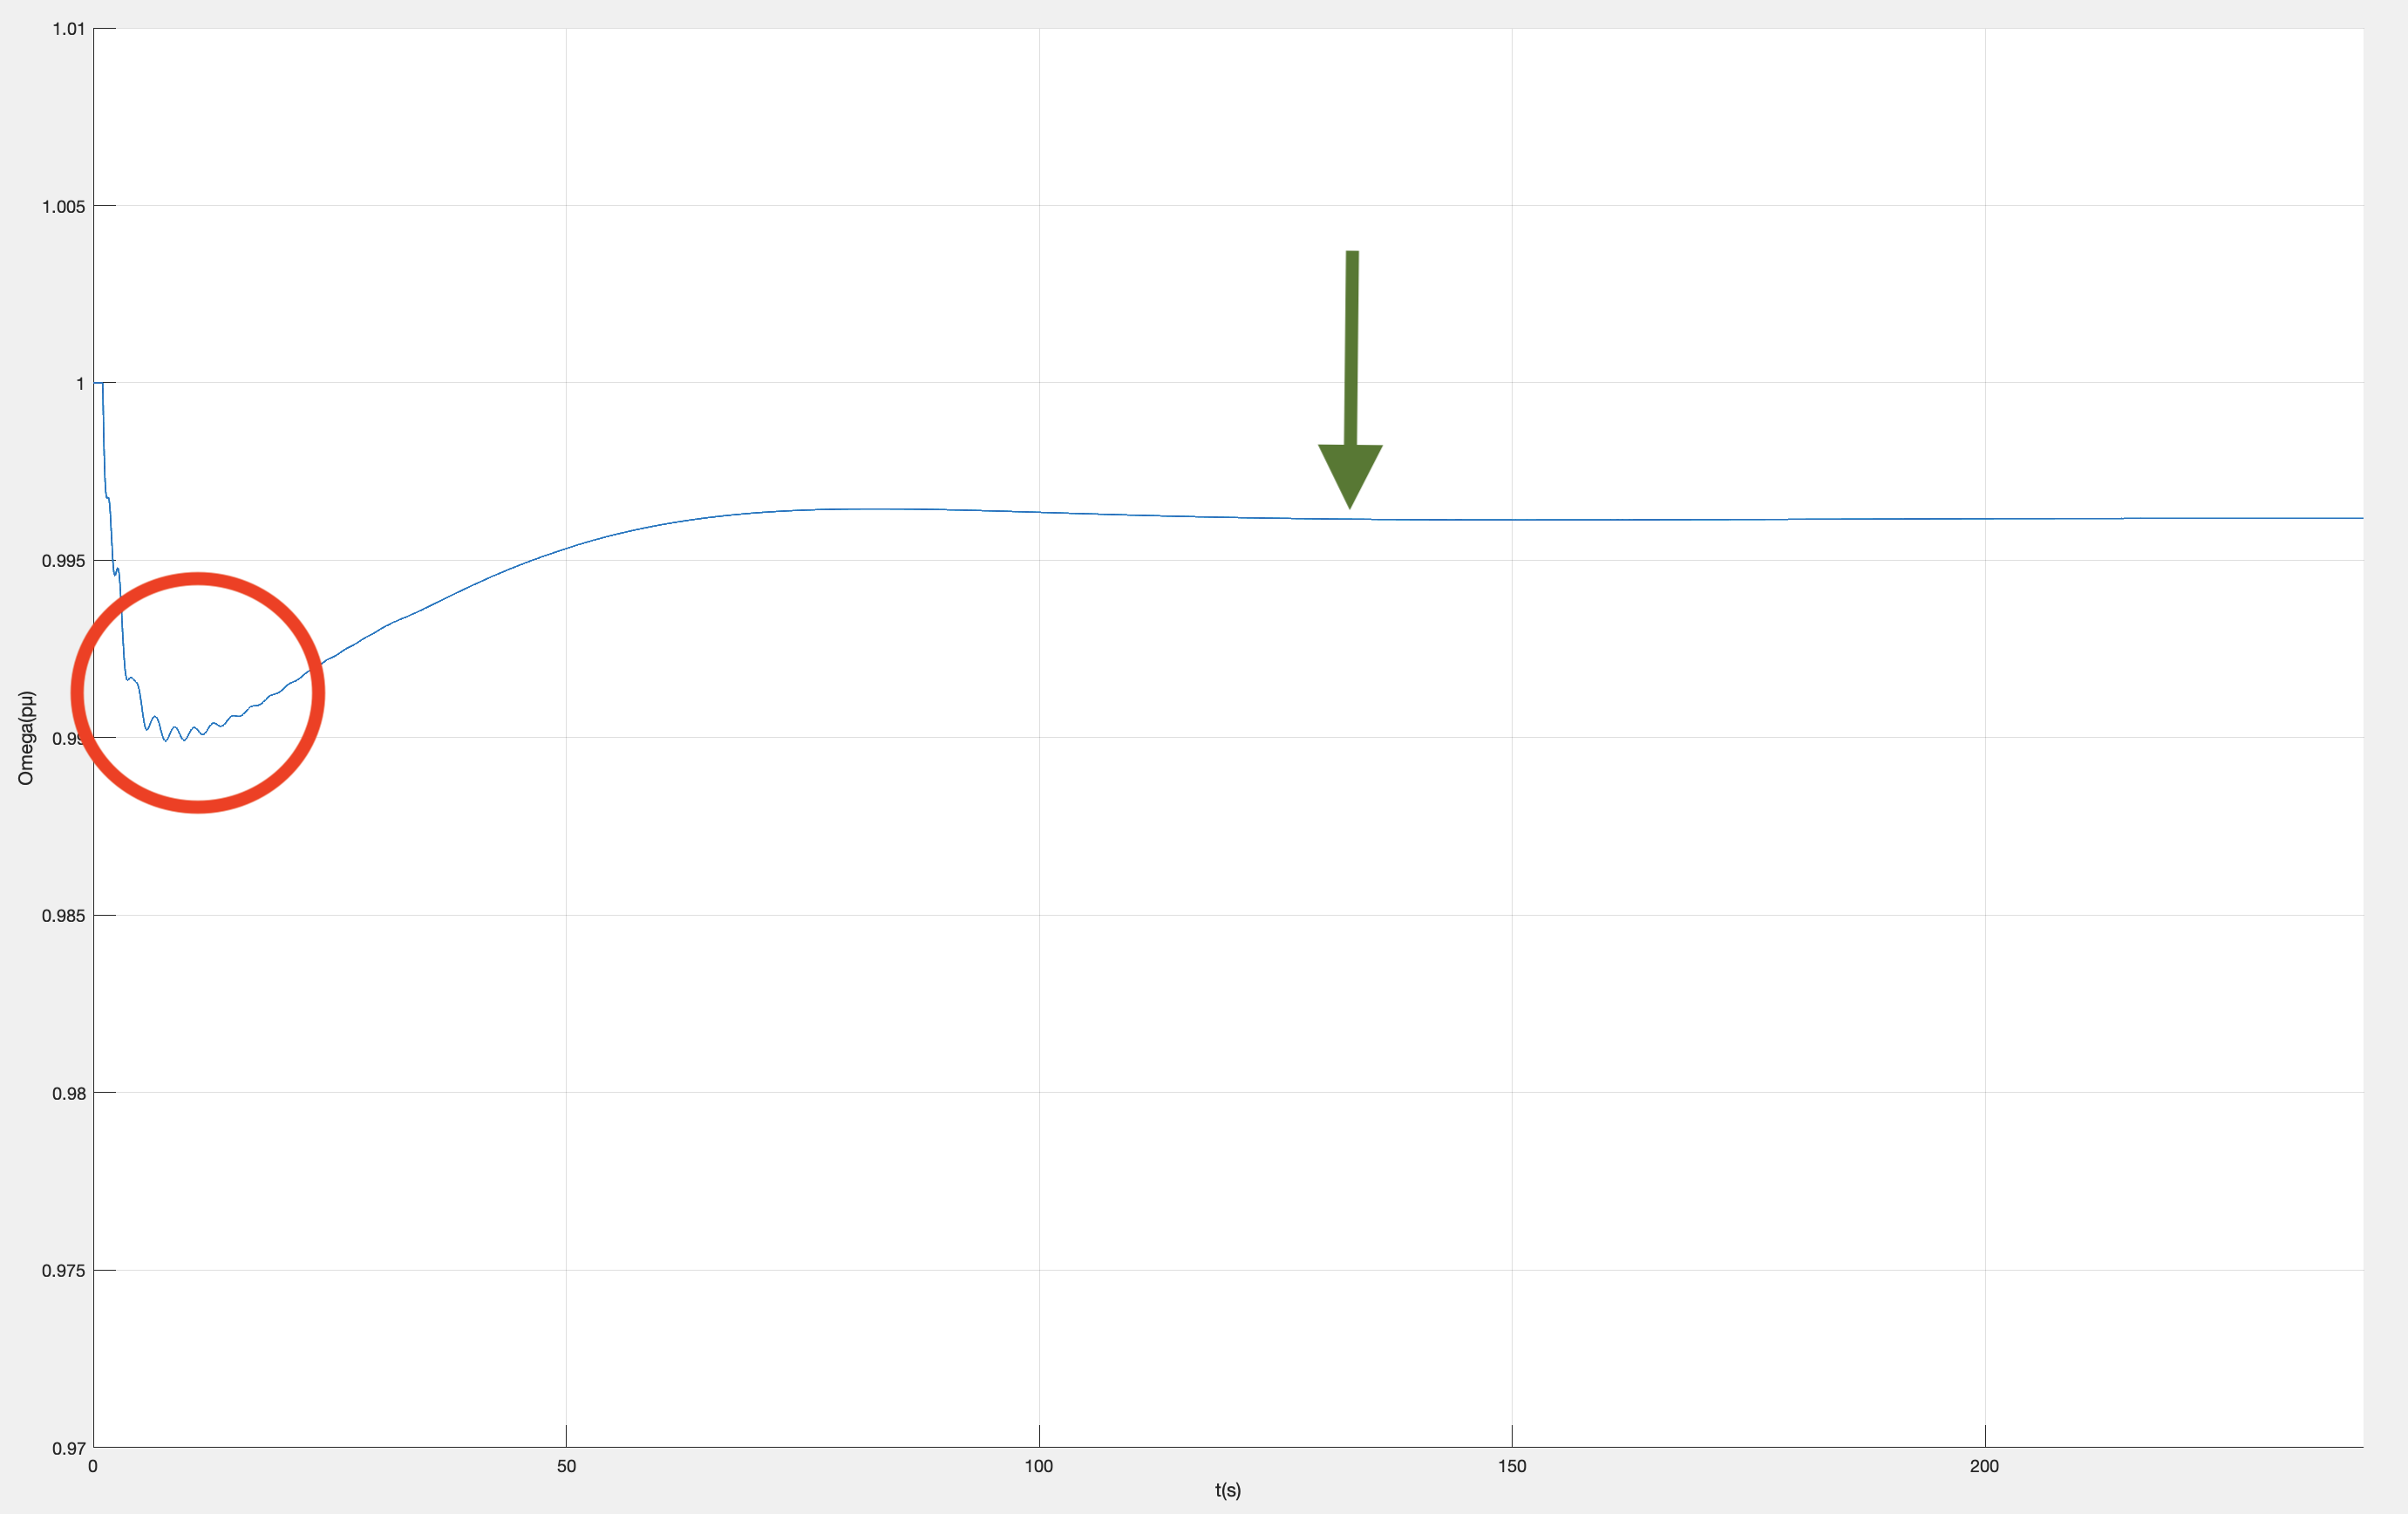
\includegraphics[scale=0.3]{figure/3_2_steady.png}
\caption{Steady-state error and high frequency component in a signal.}
\label{3_2_steady}
\end{figure}

In reality, whatever it is the automobile control system, the electronic compass control system or the Automatic Generation Control, the steady-state errors occurs if we use P control only. 

We introduce the I-term to remove such a steady-state error. Briefly, the integral of the error accumulate the previous errors and the I-term is proportional to the integral of the error, which means the I-term is proportional to previous accumulated errors. The integral of the error will not be zero, unless the error is removed. Gradually, the controlled signal will be larger and the new signal will approach to the nominal value. 

To the D-term, it is proportional to the derivative of the error. In another way, the D-term is proportional to the gradient of the signal. Thus, the D-term amplifies the high frequency component in the signal and will disturb the system. 